% =====================================================================
%  Guía de laboratorio — IEL04 — Circuitos Eléctricos I, semana 13
%  Escrita por src/guia_laboratorio.py con la plantilla institucional
%  (config/framework_iub/guia-laboratorio/: guialabiub.sty e img/, copiados a esta carpeta).
%
%  Compilar con:  pdflatex -> biber -> pdflatex -> pdflatex
%  (En Overleaf: compilador pdfLaTeX; biber se ejecuta solo.)
% =====================================================================
\documentclass[12pt]{article}

% Opciones: [sinmarca] quita la marca de agua; [borrador] muestra márgenes
%           [ieee] referencias IEEE (por defecto); [apa] referencias APA 7
\usepackage{guialabiub}

% --------------------- Diagramas de flujo del procedimiento ----------------
% (TikZ, con los mismos estilos del .tex del temario; la plantilla no los trae)
\usepackage{tikz}
\usetikzlibrary{arrows.meta,positioning,shapes.geometric,shapes.misc}
\usepackage{adjustbox}
\definecolor{iubnavy}{HTML}{121023}
\definecolor{iubyellow}{HTML}{FFDF2D}
\definecolor{iubblue}{HTML}{00ADE7}
\definecolor{iuborange}{HTML}{E39037}
\definecolor{iubgreen}{HTML}{3B9C6D}
\definecolor{iubpurple}{HTML}{8E6BBF}
\definecolor{iubgris}{HTML}{D5DAE3}
\definecolor{iubgrisoscuro}{HTML}{7C8598}
\definecolor{iubfondoazul}{HTML}{EBF7FD}
\definecolor{iubfondonaranja}{HTML}{FDF4EA}
\definecolor{iubfondoverde}{HTML}{EDF8F2}
\definecolor{iubfondogris}{HTML}{F4F6F9}
\tikzset{
  dcaja/.style={draw=iubblue, fill=iubfondoazul, line width=1pt, rounded corners=1pt, align=center, inner sep=2pt},
  destado/.style={draw=iubblue, fill=iubfondoazul, line width=1pt, rounded corners=6pt, align=center, inner sep=2pt},
  ddecision/.style={draw=iuborange, fill=iubfondonaranja, line width=1pt, diamond, aspect=1.6, align=center, inner sep=1pt},
  dterminal/.style={draw=iubgreen, fill=iubfondoverde, line width=1pt, rounded rectangle, align=center, inner sep=2pt},
  dflecha/.style={-{Stealth[length=2.4mm]}, line width=0.9pt, draw=iubnavy},
  drotulo/.style={font=\footnotesize, text=iubgrisoscuro, fill=white, fill opacity=0.92, text opacity=1, inner sep=1.5pt},
}

% --------------------------- Bibliografía ----------------------------
\addbibresource{IEL04-semana13.bib}

% --------------------------- Datos de la guía -------------------------
\facultad{Facultad de Ingenierías}
\modulo{IEL04 --- Circuitos Eléctricos I}
\docente{Ing. Sergio Martinez Castilla}

\begin{document}

% Orden de la bibliografía: el mismo del .md (biblatex numera por orden de primera cita)
\nocite{ref1,ref2,ref3}

\datosguia
\lineablanco

% Título de la práctica y ficha de la sesión
{\centering\bfseries Guía de laboratorio: Caracterización de un filtro pasabanda RLC en serie: frecuencia de resonancia, frecuencias de corte, ancho de banda y factor de calidad\par}
\lineablanco
\textbf{Semana:} 13 de 14 \quad \textbf{Resultado de aprendizaje:} IEL04-RA4 \quad \textbf{Práctica:} propuesta a partir de la bibliografía \cite{ref1}, \cite{ref2}, \cite{ref3} \quad \textbf{Duración:} \SI{240}{\minute}
\lineablanco
La práctica cierra el RA IEL04-RA4 y corresponde a la sesión teórica de la semana 13, \guillemotleft{}Cálculo y medición de parámetros en circuitos RLC en serie, en paralelo y mixtos: filtros resonantes, frecuencia de resonancia, ancho de banda y nomenclatura\guillemotright{}. Reproduce su caso de estudio: un filtro pasabanda formado por el resistor de 100 \ensuremath{\Omega}, la bobina L3 y el condensador C2 en serie, con la salida en el resistor, del que se miden la frecuencia de resonancia, las frecuencias de corte, el ancho de banda y el factor de calidad. No hay un manual de laboratorio asignado, por lo que la práctica se propone a partir de la bibliografía cargada: Floyd define el ancho de banda de los circuitos resonantes entre las frecuencias en que la respuesta cae al 70,7 \% y trata los filtros pasabanda \cite{ref1}, Boylestad el factor de calidad y la selectividad \cite{ref2} y Deorsola la nomenclatura y la simbología de los circuitos \cite{ref3}.

% ---------------------------------------------------------------------
\section{Objetivos}\label{sec:objetivos}
\textbf{Objetivo general:} Caracterizar experimentalmente un filtro pasabanda RLC en serie y contrastar sus parámetros con el cálculo.
\lineablanco
\textbf{Objetivos específicos:}
\begin{itemize}
  \item Identificar y verificar con instrumentos los componentes del filtro, con su simbología y sus unidades. \emph{(CE1)}
  \item Medir la tensión de salida del filtro en función de la frecuencia con el multímetro y el osciloscopio. \emph{(CE2)}
  \item Determinar experimentalmente la frecuencia de resonancia, las frecuencias de corte, el ancho de banda y el factor de calidad del circuito RLC en serie. \emph{(CE3)}
\end{itemize}

% ---------------------------------------------------------------------
\section{Materiales y Equipos}\label{sec:materiales}
\begin{itemize}
  \item \textbf{Resistor}: 100 \ensuremath{\Omega} (medido 99,5 \ensuremath{\Omega} en la sesión)
  \item \textbf{Bobina L3 del kit}: 103K, 10,4 mH y 24,6 \ensuremath{\Omega} medidos
  \item \textbf{Condensador C2 del kit}: 104K, 97,8 nF medidos
  \item \textbf{Generador de funciones}
  \item \textbf{Osciloscopio de dos canales con puntas \texttimes{}10}
  \item \textbf{Multímetro digital de verdadero valor eficaz} (2)
  \item \textbf{Medidor LCR}
  \item \textbf{Protoboard}
  \item \textbf{Cables de conexión} (12)
  \item \textbf{Resistencia de descarga}: 1 k\ensuremath{\Omega}
\end{itemize}

% ---------------------------------------------------------------------
\section{Procedimiento}\label{sec:procedimiento}
La práctica ocupa el bloque de 2 h de laboratorio de la sesión y se realiza en grupos de tres estudiantes, con tres roles que rotan entre etapas: quien monta y opera el circuito, quien mide y quien registra y verifica los cálculos. Antes de energizar cualquier montaje, el docente o el monitor revisa la conexión. Cada etapa abre con su diagrama de flujo, que muestra la secuencia y las comprobaciones de un vistazo, y sigue con sus pasos numerados; cada paso indica cuánto dura, qué debe observarse para saber que salió bien y qué hacer si no. Los valores numéricos de la sesión teórica sirven de referencia: las lecturas propias del grupo se registran en las tablas de la sección de análisis.
\lineablanco
% --- Etapa 1: Preparación y predicción (4 pasos) ---
\subsection{Preparación y predicción (\SI{29}{\minute})}\label{sec:etapa-1}
% --- Figura 1: diagrama de flujo de la etapa 1 (TikZ; misma disposición que el PNG del .md) ---
\begin{figure}[H]
  \centering
\begin{adjustbox}{max width=\linewidth}
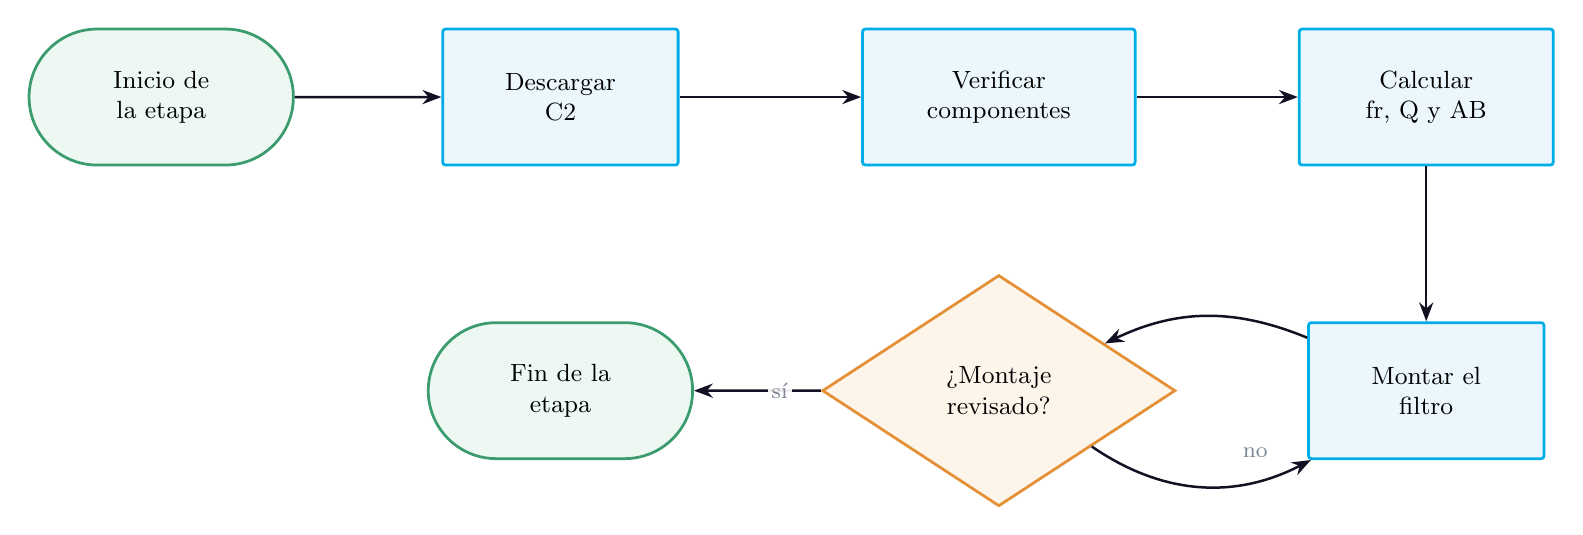
\begin{tikzpicture}[x=1in, y=1in, font=\small]
  % nodos (centro en pulgadas, con el tamano que calcula figuras.py)
  \node[dterminal, minimum width=1.377in, minimum height=0.680in] (n0) at (0.689,-0.340) {Inicio de \\ la etapa};  % ini
  \node[dcaja, minimum width=1.177in, minimum height=0.680in] (n1) at (2.685,-0.340) {Descargar \\ C2};  % a0
  \node[dcaja, minimum width=1.363in, minimum height=0.680in] (n2) at (4.877,-0.340) {Verificar \\ componentes};  % a1
  \node[dcaja, minimum width=1.270in, minimum height=0.680in] (n3) at (7.014,-0.340) {Calcular \\ fr, Q y AB};  % a2
  \node[dcaja, minimum width=1.177in, minimum height=0.680in] (n4) at (7.014,-1.808) {Montar el \\ filtro};  % a3
  \node[ddecision, minimum width=1.766in, minimum height=1.156in] (n5) at (4.877,-1.808) {\textquestiondown{}Montaje \\ revisado?};  % dec
  \node[dterminal, minimum width=1.377in, minimum height=0.680in] (n6) at (2.685,-1.808) {Fin de la \\ etapa};  % fin
  % flechas (las de retorno, curvas)
  \draw[dflecha] (n0) -- (n1);
  \draw[dflecha] (n1) -- (n2);
  \draw[dflecha] (n2) -- (n3);
  \draw[dflecha] (n3) -- (n4);
  \draw[dflecha] (n4) to[bend right=24] (n5);
  \draw[dflecha] (n5) -- (n6);
  \draw[dflecha] (n5) to[bend right=31] (n4);
  % rotulos de las flechas (donde los pone el PNG: sin caer sobre un nodo)
  \node[drotulo] at (3.781,-1.808) {sí};
  \node[drotulo] at (6.159,-2.116) {no};
\end{tikzpicture}
\end{adjustbox}
  \caption{Diagrama de flujo de la etapa 1: Preparación y predicción}
  \label{fig:flujo-1}
\end{figure}
\begin{pasos}
  \item \textbf{Paso~1:} Descargar el condensador conectando entre sus terminales, durante unos segundos, una resistencia de 1 k\ensuremath{\Omega} sujeta con pinzas aisladas, y medir con el voltímetro en cd la tensión entre terminales. \emph{(aprox.~\SI{3}{\minute})} \textbf{Comprobación:} La tensión debe ser prácticamente nula (menos de 0,1 V); si no lo es, repetir la descarga antes de manipular el componente. \textbf{Seguridad:} No cortocircuitar los terminales con los dedos ni con una herramienta metálica: un condensador puede conservar carga después de desconectado.
  \item \textbf{Paso~2:} Verificar el resistor con el ohmímetro, la bobina L3 con el medidor LCR y el ohmímetro (10,4 mH y 24,6 \ensuremath{\Omega} esperados) y el condensador C2 con el medidor LCR (97,8 nF esperados). \emph{(aprox.~\SI{8}{\minute})} \textbf{Comprobación:} Si algún valor difiere más que su tolerancia del registrado, anotar el nuevo valor y rehacer el cálculo previo con él.
  \item \textbf{Paso~3:} Calcular con los valores medidos la frecuencia de resonancia, el factor de calidad con la resistencia total del lazo $R + R_W$, las frecuencias de corte y el ancho de banda $AB = f_r/Q$. \emph{(aprox.~\SI{12}{\minute})} \textbf{Comprobación:} Deben obtenerse $f_r$ cerca de 4990 Hz, Q cerca de 2,6 y un ancho de banda cercano a 1900 Hz.
  \item \textbf{Paso~4:} Montar en serie el resistor, L3 y C2, con el resistor del lado de tierra para medir en él la salida. \emph{(aprox.~\SI{6}{\minute})} \textbf{Comprobación:} El docente revisa el montaje antes de energizar. \textbf{Seguridad:} Montar con el generador apagado.
\end{pasos}
% --- Etapa 2: Resonancia del filtro (3 pasos) ---
\subsection{Resonancia del filtro (\SI{22}{\minute})}\label{sec:etapa-2}
% --- Figura 2: diagrama de flujo de la etapa 2 (TikZ; misma disposición que el PNG del .md) ---
\begin{figure}[H]
  \centering
\begin{adjustbox}{max width=\linewidth}
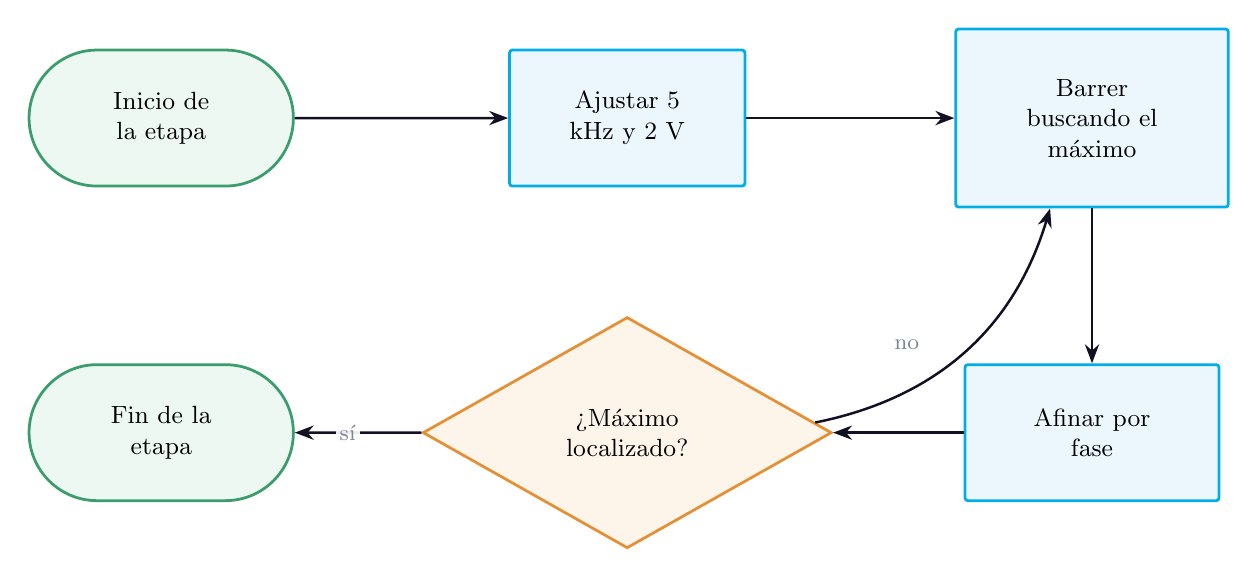
\begin{tikzpicture}[x=1in, y=1in, font=\small]
  % nodos (centro en pulgadas, con el tamano que calcula figuras.py)
  \node[dterminal, minimum width=1.377in, minimum height=0.680in] (n0) at (0.689,-0.445) {Inicio de \\ la etapa};  % ini
  \node[dcaja, minimum width=1.177in, minimum height=0.680in] (n1) at (3.019,-0.445) {Ajustar 5 \\ kHz y 2 V};  % a0
  \node[dcaja, minimum width=1.363in, minimum height=0.890in] (n2) at (5.343,-0.445) {Barrer \\ buscando el \\ máximo};  % a1
  \node[dcaja, minimum width=1.270in, minimum height=0.680in] (n3) at (5.343,-2.018) {Afinar por \\ fase};  % a2
  \node[ddecision, minimum width=2.045in, minimum height=1.156in] (n4) at (3.019,-2.018) {\textquestiondown{}Máximo \\ localizado?};  % dec
  \node[dterminal, minimum width=1.377in, minimum height=0.680in] (n5) at (0.689,-2.018) {Fin de la \\ etapa};  % fin
  % flechas (las de retorno, curvas)
  \draw[dflecha] (n0) -- (n1);
  \draw[dflecha] (n1) -- (n2);
  \draw[dflecha] (n2) -- (n3);
  \draw[dflecha] (n3) -- (n4);
  \draw[dflecha] (n4) -- (n5);
  \draw[dflecha] (n4) to[bend right=31] (n2);
  % rotulos de las flechas (donde los pone el PNG: sin caer sobre un nodo)
  \node[drotulo] at (1.621,-2.018) {sí};
  \node[drotulo] at (4.417,-1.580) {no};
\end{tikzpicture}
\end{adjustbox}
  \caption{Diagrama de flujo de la etapa 2: Resonancia del filtro}
  \label{fig:flujo-2}
\end{figure}
\begin{pasos}
  \item \textbf{Paso~5:} Ajustar el generador a una onda sinusoidal de 5 kHz y medir con el osciloscopio y con el multímetro de verdadero valor eficaz que la tensión en los bornes del circuito, con el circuito conectado, sea de 2,00 V eficaces. \emph{(aprox.~\SI{6}{\minute})} \textbf{Comprobación:} El multímetro debe indicar 2,00 V y el osciloscopio una sinusoide sin distorsión; si la tensión baja al conectar el circuito, reajustar la amplitud con el circuito conectado.
  \item \textbf{Paso~6:} Barrer la frecuencia buscando el máximo de la tensión en el resistor, reajustando la entrada a 2,00 V eficaces a cada frecuencia. \emph{(aprox.~\SI{8}{\minute})} \textbf{Comprobación:} El máximo debe estar cerca de 5 kHz y por debajo de 2,00 V por la resistencia de devanado.
  \item \textbf{Paso~7:} Afinar la resonancia por fase con el osciloscopio (tensión del resistor en fase con la de la fuente) y anotar $f_r$ y la tensión de salida máxima. \emph{(aprox.~\SI{8}{\minute})} \textbf{Comprobación:} La tensión de salida máxima esperada es cercana a 1,60 V.
\end{pasos}
% --- Etapa 3: Frecuencias de corte y ancho de banda (4 pasos) ---
\subsection{Frecuencias de corte y ancho de banda (\SI{28}{\minute})}\label{sec:etapa-3}
% --- Figura 3: diagrama de flujo de la etapa 3 (TikZ; misma disposición que el PNG del .md) ---
\begin{figure}[H]
  \centering
\begin{adjustbox}{max width=\linewidth}
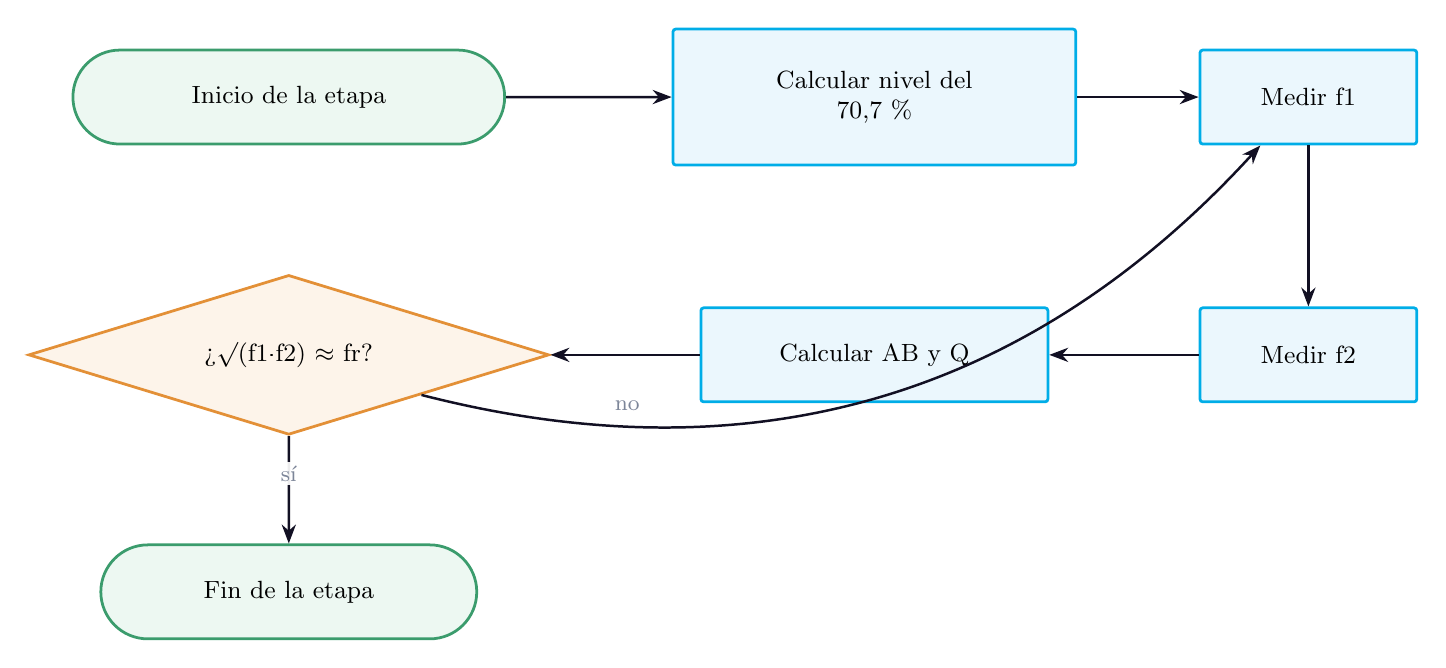
\begin{tikzpicture}[x=1in, y=1in, font=\small]
  % nodos (centro en pulgadas, con el tamano que calcula figuras.py)
  \node[dterminal, minimum width=2.214in, minimum height=0.470in] (n0) at (1.301,-0.340) {Inicio de la etapa};  % ini
  \node[dcaja, minimum width=2.014in, minimum height=0.680in] (n1) at (4.229,-0.340) {Calcular nivel del \\ 70,7 \%};  % a0
  \node[dcaja, minimum width=1.084in, minimum height=0.470in] (n2) at (6.399,-0.340) {Medir f1};  % a1
  \node[dcaja, minimum width=1.084in, minimum height=0.470in] (n3) at (6.399,-1.629) {Medir f2};  % a2
  \node[dcaja, minimum width=1.735in, minimum height=0.470in] (n4) at (4.229,-1.629) {Calcular AB y Q};  % a3
  \node[ddecision, minimum width=2.603in, minimum height=0.799in] (n5) at (1.301,-1.629) {\textquestiondown{}\ensuremath{\surd}(f1\textperiodcentered{}f2) \ensuremath{\approx} fr?};  % dec
  \node[dterminal, minimum width=1.935in, minimum height=0.470in] (n6) at (1.301,-2.814) {Fin de la etapa};  % fin
  % flechas (las de retorno, curvas)
  \draw[dflecha] (n0) -- (n1);
  \draw[dflecha] (n1) -- (n2);
  \draw[dflecha] (n2) -- (n3);
  \draw[dflecha] (n3) -- (n4);
  \draw[dflecha] (n4) -- (n5);
  \draw[dflecha] (n5) -- (n6);
  \draw[dflecha] (n5) to[bend right=31] (n2);
  % rotulos de las flechas (donde los pone el PNG: sin caer sobre un nodo)
  \node[drotulo] at (1.301,-2.222) {sí};
  \node[drotulo] at (2.993,-1.885) {no};
\end{tikzpicture}
\end{adjustbox}
  \caption{Diagrama de flujo de la etapa 3: Frecuencias de corte y ancho de banda}
  \label{fig:flujo-3}
\end{figure}
\begin{pasos}
  \item \textbf{Paso~8:} Calcular el 70,7 \% de la tensión de salida máxima \cite{ref1}. \emph{(aprox.~\SI{2}{\minute})} \textbf{Comprobación:} Con 1,60 V de máximo, el nivel de corte es de unos 1,13 V.
  \item \textbf{Paso~9:} Bajar la frecuencia desde $f_r$ hasta que la salida caiga a ese nivel, reajustando la entrada, y anotar $f_1$. \emph{(aprox.~\SI{10}{\minute})} \textbf{Comprobación:} $f_1$ debe estar cerca de 4,1 kHz.
  \item \textbf{Paso~10:} Subir la frecuencia desde $f_r$ hasta el mismo nivel y anotar $f_2$. \emph{(aprox.~\SI{10}{\minute})} \textbf{Comprobación:} $f_2$ debe estar cerca de 6,0 kHz.
  \item \textbf{Paso~11:} Calcular $AB = f_2 - f_1$, $Q = f_r/AB$ y la comprobación $\sqrt{f_1 f_2}$, que debe coincidir con $f_r$. \emph{(aprox.~\SI{6}{\minute})} \textbf{Comprobación:} Si $\sqrt{f_1 f_2}$ se aparta más del 2 \% de $f_r$, repetir la medición de la frecuencia de corte más dudosa.
\end{pasos}
% --- Etapa 4: Desmontaje y cierre (3 pasos) ---
\subsection{Desmontaje y cierre (\SI{10}{\minute})}\label{sec:etapa-4}
% --- Figura 4: diagrama de flujo de la etapa 4 (TikZ; misma disposición que el PNG del .md) ---
\begin{figure}[H]
  \centering
\begin{adjustbox}{max width=\linewidth}
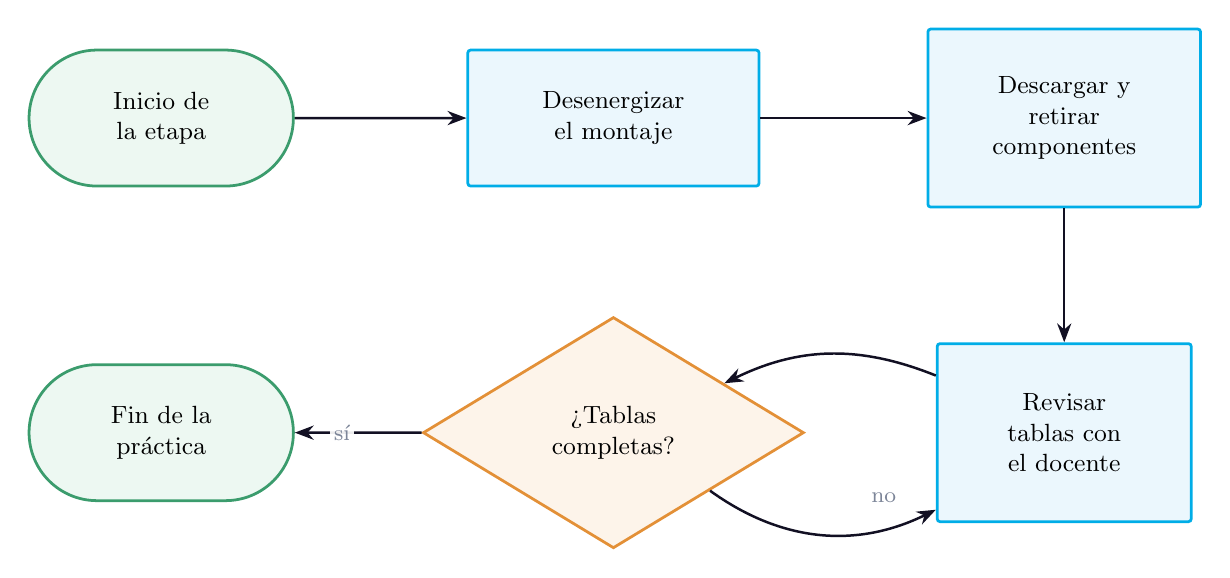
\begin{tikzpicture}[x=1in, y=1in, font=\small]
  % nodos (centro en pulgadas, con el tamano que calcula figuras.py)
  \node[dterminal, minimum width=1.377in, minimum height=0.680in] (n0) at (0.689,-0.445) {Inicio de \\ la etapa};  % ini
  \node[dcaja, minimum width=1.456in, minimum height=0.680in] (n1) at (2.950,-0.445) {Desenergizar \\ el montaje};  % a0
  \node[dcaja, minimum width=1.363in, minimum height=0.890in] (n2) at (5.204,-0.445) {Descargar y \\ retirar \\ componentes};  % a1
  \node[dcaja, minimum width=1.270in, minimum height=0.890in] (n3) at (5.204,-2.018) {Revisar \\ tablas con \\ el docente};  % a2
  \node[ddecision, minimum width=1.905in, minimum height=1.156in] (n4) at (2.950,-2.018) {\textquestiondown{}Tablas \\ completas?};  % dec
  \node[dterminal, minimum width=1.377in, minimum height=0.680in] (n5) at (0.689,-2.018) {Fin de la \\ práctica};  % fin
  % flechas (las de retorno, curvas)
  \draw[dflecha] (n0) -- (n1);
  \draw[dflecha] (n1) -- (n2);
  \draw[dflecha] (n2) -- (n3);
  \draw[dflecha] (n3) to[bend right=24] (n4);
  \draw[dflecha] (n4) -- (n5);
  \draw[dflecha] (n4) to[bend right=31] (n3);
  % rotulos de las flechas (donde los pone el PNG: sin caer sobre un nodo)
  \node[drotulo] at (1.593,-2.018) {sí};
  \node[drotulo] at (4.302,-2.343) {no};
\end{tikzpicture}
\end{adjustbox}
  \caption{Diagrama de flujo de la etapa 4: Desmontaje y cierre}
  \label{fig:flujo-4}
\end{figure}
\begin{pasos}
  \item \textbf{Paso~12:} Apagar el generador de funciones y la fuente, desconectar las puntas del osciloscopio y retirar la alimentación del protoboard. \emph{(aprox.~\SI{3}{\minute})} \textbf{Comprobación:} Ningún indicador de salida debe quedar encendido en el generador ni en la fuente. \textbf{Seguridad:} Desenergizar siempre antes de retirar componentes.
  \item \textbf{Paso~13:} Descargar los condensadores del montaje con la resistencia de descarga, retirar los componentes y devolverlos al kit del grupo con su rótulo. \emph{(aprox.~\SI{4}{\minute})} \textbf{Comprobación:} El kit debe quedar completo, con cada componente en su lugar y con su valor medido anotado.
  \item \textbf{Paso~14:} Revisar con el docente las tablas de registro antes de abandonar el banco. \emph{(aprox.~\SI{3}{\minute})} \textbf{Comprobación:} Las tablas deben estar completas y con unidades; si falta un dato, repetir esa medición antes de desmontar el instrumento.
\end{pasos}

% ---------------------------------------------------------------------
\section{Cuestiones a Resolver}\label{sec:cuestiones}
\begin{enumerate}
  \item \textquestiondown{}Por qué la tensión de salida en la resonancia no alcanza la tensión de la fuente?
  \item \textquestiondown{}Qué diferencia hay entre el factor de calidad medido y el que predice el cálculo ideal con valores nominales, y a qué se debe?
  \item \textquestiondown{}Qué ocurriría con el ancho de banda si la tensión se fijara en el dial del generador y no en los bornes del circuito?
  \item \textquestiondown{}Qué componente habría que cambiar para hacer el filtro más selectivo, y en qué sentido?
  \item \textquestiondown{}Por qué $\sqrt{f_1 f_2}$ sirve para comprobar la coherencia de las tres frecuencias medidas?
\end{enumerate}

% ---------------------------------------------------------------------
\section{Análisis de Resultados}\label{sec:analisis}
Presentar en la tabla de registro los parámetros del filtro calculados de forma ideal con valores nominales, calculados con valores medidos y resistencia de devanado, y medidos, con la diferencia porcentual respecto del cálculo con valores medidos.
\lineablanco
Registrar la tensión de salida a unas diez frecuencias entre 2 kHz y 10 kHz y graficarla contra la frecuencia en escala logarítmica, marcando $f_r$, $f_1$, $f_2$ y el nivel del 70,7 \%.
% --- Tabla 1: Parámetros del filtro pasabanda RLC en serie (6 filas vacías para registrar en el banco) ---
\begin{table}[H]
  \centering
  \caption{Parámetros del filtro pasabanda RLC en serie}
  \label{tab:registro-1}
  \begin{tabularx}{\linewidth}{>{\raggedright\arraybackslash}X>{\raggedright\arraybackslash}X>{\raggedright\arraybackslash}X>{\raggedright\arraybackslash}X>{\raggedright\arraybackslash}X>{\raggedright\arraybackslash}X}
    \toprule
    \textbf{Parámetro} & \textbf{Ideal nominal} & \textbf{Cálculo con medidos} & \textbf{Medido} & \textbf{Unidad} & \textbf{Diferencia (\%)} \\
    \midrule
    \rule{0pt}{0.8cm} & & & & & \\
    \cmidrule(lr){1-6}
    \rule{0pt}{0.8cm} & & & & & \\
    \cmidrule(lr){1-6}
    \rule{0pt}{0.8cm} & & & & & \\
    \cmidrule(lr){1-6}
    \rule{0pt}{0.8cm} & & & & & \\
    \cmidrule(lr){1-6}
    \rule{0pt}{0.8cm} & & & & & \\
    \cmidrule(lr){1-6}
    \rule{0pt}{0.8cm} & & & & & \\
    \bottomrule
  \end{tabularx}
\end{table}
% --- Tabla 2: Respuesta en frecuencia del filtro (10 filas vacías para registrar en el banco) ---
\begin{table}[H]
  \centering
  \caption{Respuesta en frecuencia del filtro}
  \label{tab:registro-2}
  \begin{tabularx}{\linewidth}{>{\raggedright\arraybackslash}X>{\raggedright\arraybackslash}X>{\raggedright\arraybackslash}X>{\raggedright\arraybackslash}X}
    \toprule
    \textbf{Frecuencia (kHz)} & \textbf{Vent (V)} & \textbf{Vsal (V)} & \textbf{Vsal/Vent} \\
    \midrule
    \rule{0pt}{0.8cm} & & & \\
    \cmidrule(lr){1-4}
    \rule{0pt}{0.8cm} & & & \\
    \cmidrule(lr){1-4}
    \rule{0pt}{0.8cm} & & & \\
    \cmidrule(lr){1-4}
    \rule{0pt}{0.8cm} & & & \\
    \cmidrule(lr){1-4}
    \rule{0pt}{0.8cm} & & & \\
    \cmidrule(lr){1-4}
    \rule{0pt}{0.8cm} & & & \\
    \cmidrule(lr){1-4}
    \rule{0pt}{0.8cm} & & & \\
    \cmidrule(lr){1-4}
    \rule{0pt}{0.8cm} & & & \\
    \cmidrule(lr){1-4}
    \rule{0pt}{0.8cm} & & & \\
    \cmidrule(lr){1-4}
    \rule{0pt}{0.8cm} & & & \\
    \bottomrule
  \end{tabularx}
\end{table}

% ---------------------------------------------------------------------
\section{Conclusiones}\label{sec:conclusiones}
Concluir si los parámetros medidos del filtro coinciden con el cálculo que usa los valores medidos y la resistencia de devanado, y por qué el cálculo ideal se aparta; relacionar la práctica con los criterios de medición en circuitos RLC del RA y con la selección de componentes de un filtro.
\lineablanco
\begin{itemize}
  \item \textquestiondown{}Qué parámetro del filtro fue más sensible a la resistencia de devanado?
  \item \textquestiondown{}Qué tan coherentes resultaron las tres frecuencias medidas?
  \item \textquestiondown{}Qué cambio de componentes propondrían para estrechar el ancho de banda?
\end{itemize}

% ---------------------------------------------------------------------
\section{Recomendaciones de Seguridad}\label{sec:seguridad}
\begin{itemize}
  \item Trabajar con el circuito desenergizado mientras se conecta o modifica el montaje; energizar solo después de la revisión del docente.
  \item Mantener la tensión de la fuente en 2,00 V eficaces: en la resonancia en serie la tensión en la bobina y en el condensador supera varias veces la de la fuente \cite{ref1}.
  \item Conectar las tierras de las dos puntas del osciloscopio a un mismo nodo de referencia: unirlas a nodos distintos cortocircuita el elemento que queda entre ellas.
\end{itemize}

% ---------------------------------------------------------------------
\section{Bibliografía}\label{sec:bibliografia}
% Las fuentes cargadas se citan en el texto con \cite{refN}; el \nocite del principio fija su orden y \nocite{*} incluye las demás del .bib.
\nocite{*}
\bibliografia

\end{document}
